\begin{problem}[\(5\)-lemma]
  Given a commutative diagram with exact rows
  \[
    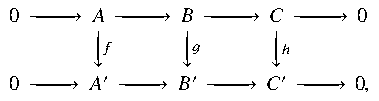
\includegraphics{ma598-ag-1-1}
  \]
  suppose \(f\) and \(h\) are isomorphisms. Prove that \(g\) is an
  isomorphism.
\end{problem}
\begin{solution}

\end{solution}
\newpage

\begin{problem}[Snake lemma]
  Given the diagram with exact rows
  \[
    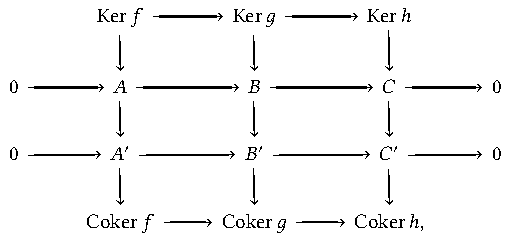
\includegraphics{ma598-ag-1-2}
  \]
  show that the sequence
  \[
    0\too
    \Ker f\too
    \Ker g\too
    \Ker h\too
    \Coker f\too
    \Coker f\too
    \Coker h\too
    0
  \]
  is exact.
\end{problem}
\begin{solution}
\end{solution}
\newpage

\begin{problem}
  Given an exact sequence of modules
  \[
    0\too A\too B\too C\too 0
  \]
  fix any \(M\in\RMod{R}\).
  \begin{enumerate}[label=(\alph*)]
  \item Show that
    \[
      0\too \Hom(M,A)\too\Hom(M,B)\too\Hom(M,C)
    \]
    is exact.
  \item Show that
    \[
      0\too \Hom(C,M)\too\Hom(B,M)\too\Hom(A,M)
    \]
    is exact.
  \end{enumerate}
\end{problem}
\begin{solution}
\end{solution}
\newpage

\begin{problem}
  A short exact sequence
  \[
    0\too A\too B\xrightarrow{\,\,p\,\,} 0
  \]
  splits if there is a homomorphism \(s\colon C\to B\) called the
  \emph{splitting} such that \(p\circ s=\id_C\). In which case, we can put
  \[
    0\too\Hom(C,M)\too\Hom(B,M)\too\Hom(A,M)\too 0
  \]
  and
  \[
    0\too\Hom(M,A)\too\Hom(M,B)\too\Hom(M,C)\too 0.
  \]
\end{problem}
\begin{solution}
\end{solution}
\newpage

\begin{problem}
  Find an example which shows that \(\Hom(\blank,M)\) is \emph{not} exact.
\end{problem}
\begin{solution}
  Consider the following example: let \(A=B=M=\bfZ\) and \(C=\bfZ/2\bfZ\)
  then the sequence
  \[
    0\too\bfZ\xrightarrow{\,\,f=2\,\,}\bfZ\too\bfZ/2\bfZ\too 0
  \]
  is exact, however Hom
\end{solution}

%%% Local Variables:
%%% mode: latex
%%% TeX-master: "../MA598-AG-Current-HW"
%%% End:
